\mychapter{Synchronous Relaxation}

\section{Introduction}
The first parallel KMC algorithm we studied was the synchronous relaxation algorithm (SR). The Synchronous Relaxation algorithm was first used to study circuit switched networks. Researchers like Lubachevsky then applied the algorithm to the Ising model and showed that are given a number of weak assumptions, the algorithm is efficient and scalable. The SR algorithm was later adapted by researchers at the University of Toledo to model thin film growth.

The Synchronous Relaxation algorithm is an optimistic algorithm which means that processors can process information independent of each other.
The algorithm works as follows:
\begin{description}
\myitem{Step 1} Each Processor generates KMC events independent of other processors for a cycle time T
\myitem{Step 2} When T expires each processor exchanges information on events that happened to see if any events generated by its neighbor affect it.
\myitem{Step 3} If events in each processor do not affect events in neighbors process, all  processors proceed to the next cycle
\myitem{Step 4} If information received from one neighboring process affects another processor, all processors redo their KMC events incorporating  information gathered.
\myitem{Step 5} Processors again exchange information if events in neighboring processes affect other neighbors Step 4 is repeated. Or else all processors go to next cycle
\end{description}~\cite{ae:kmc}

\begin{figure}
\hrule
\resizebox{\textwidth}{!}{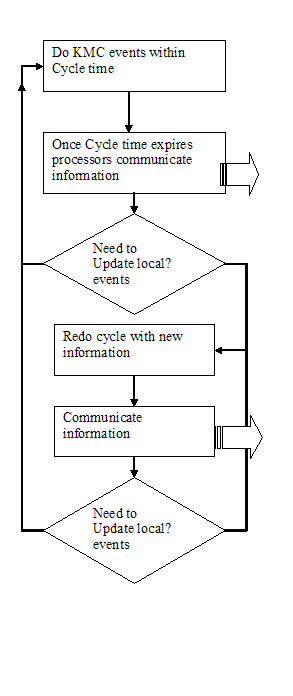
\includegraphics{srright}
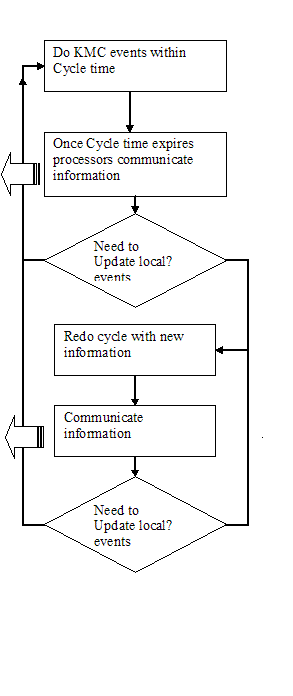
\includegraphics{srleft}}
\hrule
\caption{Synchronous Relaxation Flow Chart}
\end{figure}

\section{Original Algorithm}

\subsection{Boundary Events}
The main problem with parallelizing lattice based KMC problems like thin film growth is that of boundary events. Boundary events are those events that take place on the edge of the lattice and may affect the evolution of neighboring lattices. The SR algorithm is used to try and iteratively correct such errors.

\subsection{Ghost Region}
The ghost region is the area of a lattice that belongs to another lattice but whose events may affect the current lattice. In the initial implementation for the fractal model the Ghost region was one lattice step since diffusions take one step at time.

\subsection{Data Structures}
Modeling KMC events using Lattices can be rather complex. This is because a number of different data structures are required to keep track of the system.

\small{\begin{description}
\myitem{\texttt{h[x][y]}} 2x2 Integer array for the height map. (Appendix \ref{code:sr/lattice.h})
\myitem{\texttt{indexa[size],ipointa[size],indexc[size]}} Three lists to keep track of mobile monomers on the lattice. (Appendix \ref{code:sr/lattice.h})
\myitem{\texttt{myeventlist[size*size]}} An event list to track. (Appendix \ref{code:sr/lattice.h})
\myitem{\texttt{bdyeventlist[size]}} Keeps track of boundary events generated. (Appendix \ref{code:sr/lattice.h})
\myitem{\texttt{ranlist[size]}} list of random numbers generated. (Appendix \ref{code:sr/lattice.h})
\end{description}}

\subsection{Functions}
\begin{description}
\myitem{\texttt{DoKMC}} using a counter this function selected the next random number from the list and used this number to determine which event should take place (diffuse or deposit)
\myitem{\texttt{CalcTime}} calculates the time increment $DT=log(Rand)/sum(event rates)$ and increments the time. It is always called after \texttt{DoKMC()}.
\myitem{\texttt{Diffuse}} This function was called by the \texttt{DoKMC()} function when a diffuse event was selected. The function selects a random location on the lattice and increments it by one. It then calls \texttt{upnbhd()}.
\myitem{\texttt{Deposit}} This function was called by the \texttt{DoKMC()} function when a deposit event was selected. The function selects a random location on the lattice and increments it by one. It then calls \texttt{upnbhd()}.
\myitem{\texttt{Upnbhd}} When a monomer moves (diffuses) or is first deposited this function is called to check whether there are any neighboring monomers or islands that would bind the monomer to the lattice. If there are no monomers or islands surrounding the current monomer then it is added to the list. If there is a monomer/island next to the list then the monomer is deleted from the list or not added in the case of a deposition. If the monomer binds with another monomer that other monomer too will be deleted.
\myitem{\texttt{Undoevent}} This is used in the SR algorithm to undo the events that occurred and restore the list and lattice their state at the beginning of the cycle.
\myitem{\texttt{BufferSendrecv}} This function communicates boundary events to neighboring processes.
\myitem{\texttt{UpdateBuffer}} This function uses boundary events received to correct the lattice. It takes the boundary events received at executes them in order of the time.
\end{description}

\section{Improvements}

\subsection{Multiple Files}
The initial algorithm was implemented in a single C file with a very large number of global variables as well as a large number of functions. To abstract different aspects of the program such as communication functions like buffersendrecv or lattice manipulation functions like diffuse or deposit, we split the program into different files. The function headers where contained in the header files such as \texttt{lattice.h} (Appendix \ref{code:sr/lattice.h}) and implemented in \texttt{lattice.cpp} (Appendix \ref{code:sr/lattice.cpp}) and \texttt{comm.cpp} (Appendix \ref{code:sr/comm.cpp} files.

\subsection{Readability}
In order to work on the existing code we had received we needed to get it more readable. To make it more readable, we first eliminated all global variables. We did this by encapsulating them in a Lattice structure and then passing this structure to functions by reference. This allowed us to follow the execution of the program easier as well add new capabilities to it.

\subsection{Function Overheads}
One of the issues slowing down the execution of the program was excessive function calls. This was taking place especially in the \texttt{Upnbhd()} function where a single call from \texttt{Upnbhd()} would call a helper function eight or more times. By making the small functions inline this helped reduce execution time.
Rewinding to first boundary event

One of the main problems with the initial implementation is that when the program entered the correction phase it had to return to the beginning of the cycle as opposed to correcting after the first boundary event. This therefore increased the computation time and cut the parallel efficiency of the program.
In order to make it possible for the program to rewind to the first boundary event, all changes made to the monomer lists would have to be recorded and then undone. This meant adding extra data structure known as \texttt{ListChange[]}. \texttt{ListChange[]}  kept track of all the insertions and deletions that took place in the monomer list. \texttt{ListChange[]} also kept track of time each of these changes occurred. When the program synchronized and tried to  correct errors from boundary events, it would loop through the \texttt{ListChange[]} structure and restore the list to the state it was at the time of the first boundary event.

\subsection{Results}
The results from the improvements we made were mixed. When function overhead was reduced, the execution time was reduced.   The results are contained in Table \ref{table:Function Overhead}

\begin{table}
\begin{tabular}{|l|l|}
\hline
Execution Time with function overhead (Sec) & Execution Time without function overhead (Sec) \\
\hline
138.16 & 109.12\\
\hline
\end{tabular}
\caption{Execution Time vs. Function Overhead}
\label{table:Function Overhead}
\end{table}

The rewind to first boundary events did not increase parallel efficiency or reduce execution time due to  the complexity of manipulating the three monomer lists. This complexity made the procedure complex and error prone. Execution time was actually increased due to these changes.   The results are contained in Table \ref{table:Rewind List}

\begin{table}
\begin{tabular}{|l|l|}
\hline
Execution Time without rewind list (Sec) & Execution Time with function overhead (Sec) \\
\hline
138.16 & 119.12\\
\hline
\end{tabular}
\caption{Execution Time vs. Rewind List usage}
\label{table:Rewind List}
\end{table}

\subsection{Analysis}
Overall the Changes made to the initial program did not adequately improve the performance of the implementation. The main factors that controlled efficiency where the cycle time, lattice size and diffusion/deposition rates.  For example reducing the cycle time to 10e-6 s with a diffusion/deposition rate of 10e6.  The results are contained in Table \ref{table:Cycle Time}

\begin{table}
\begin{tabular}{|l|l|}
\hline
Execution Time in Sec & Execution Time in Sec \\
Cycle Time=10e3 & Cycle Time=10e6 \\
Diffusion/Deposition=10e5 & Diffusion/Deposition=10e5 \\
\hline
138.16 & 90.12\\
\hline
\end{tabular}
\caption{Execution Time and Cycle time}
\label{table:Cycle Time}
\end{table}

Parallel efficiency was difficult to measure in the initial program because we relied on the OSC cluster and any requests for more than 4 processors resulted in a long queue that could take hours or weeks before a turnaround.

%\subsection{Multiple Files}
%The initial algorithm was implemented in a single C file with a very large number of global variables as well as a large number of functions. To abstract different aspects %of the program such as communication functions like buffersendrecv or lattice manipulation functions like diffuse or deposit, we split the program into different files. The %function headers where contained in the header files such as lattice.h and implemented in lattice.c and comm.c files.

%\subsection{Readability}
%In order to work on the existing code we had received we needed to get it more readable. To make it more readable, we first eliminated all global variables. We did this by %encapsulating them in a Lattice structure and then passing this structure to functions by reference. This allowed us to follow the execution of the program easier as well %add new capabilities to it.

%\subsection{Function Overheads}
%One of the issues slowing down the execution of the program was excessive function calls. This was taking place especially in the Upnbhd() function where a single call from %upnbhd would call a helper function eight or more times. By making the small functions inline this helped reduce execution time.
%Rewinding to first boundary event

%One of the main problems with the initial implementation is that when the program entered the correction phase it had to return to the beginning of the cycle as opposed to correcting after the first boundary event. This therefore increased the computation time and cut the parallel efficiency of the program.
%In order to make it possible for the program to rewind to the first boundary event, all changes made to the monomer lists would have to be recorded and then undone. This meant adding extra data structure known as listchange[]. ListChange[]  kept track of all the insertions and deletions that took place in the monomer list. ListChange[] also kept track of time each of these changes occurred. When the program synchronized and tried to  correct errors from boundary events, it would loop through the listChange[] structure and restore the list to the state it was at the time of the first boundary event.

\subsection{Implementing the Program in C++}
\subsubsection{Motivation}
The motivation for moving the algorithm from C to C++ where
\begin{enumerate}
\item It allowed for a much better abstraction of the program
\item Lattice object would allow for process-processor independence
\item The Lattice class could be reused easily in other algorithms like Time Warp
\item Easier to debug
\end{enumerate}

\subsubsection{Lattice Object}
The lattice Object was now made up of an array of Sites. Each site contained information about its location, height and if a monomer was present the location of that monomer on the monomer list.

\begin{code}{Site and Lattice Object}{sitelattice}
Class Site
\{
    int index;//location of monomer on the monomer list
    int height;
    point position;
\}

Site Lattice[X][Y];//lattice object.
\end{code}

The main advantages of this approach was that it simplified the updating of monomer lists. This meant that we could implement a rewind list easier since there is only ONE list to worry about.

\subsubsection{Multiple files}
Moving from C to C++ allowed us to further abstract the code. The lattice functions could now be separate from the communication functions. All the MPI calls were encapsulated in an easy to use \texttt{MPIWrapper} Class.

\subsubsection{Rewind List}
As mentioned earlier the rewind list class was now easier to implement since we had a single monomer list.

\subsubsection{Results and Analysis}
Using a 800 by 200 lattice we tested the parallel efficiency of the algorithm on the local cluster the results are contained in Table \ref{parallelefficiency}.  They clearly show that the performance degrades at nearly exponential rate as the number of processes increases.  This is due to the conservative nature of the algorithm, each synchronization cycle taking longer as more processes are added.  Ultimately there is a hard performance limit, as eventually the communication time will significantly outweigh any possible benefit from parallelization.

It may be possible to tune the SR algorithm with some sort of emergent heuristic algorithm to reduce or extend the cycle lengths between conservative synchronizations.  However, this would add further complication the the algorithm for what could be seen as a negligible benefit, as you're still being restrained by the conservative nature of SR.

\begin{table}
\begin{tabular}{|l|l|l|}
\hline
Num Processes & Execution Time & Parallel Efficiency \\ \hline
1 & 11.1 & 1 \\ \hline
2 & 9.233 & 0.6 \\ \hline
4 & 8.7 & 0.3 \\ \hline
5 & 8.66 & 0.25 \\ \hline
8 & 10.38 & 0.13 \\ \hline
10 & 10.23 & 0.10 \\ \hline
\end{tabular}
\caption{Execution Time and Parallel Efficiency}
\label{parallelefficiency}
\end{table}

